\documentclass[
  a4paper,            % DIN A4
  DIV=10,             % Schriftgröße und Satzspiegel
  oneside,            % einseitiger Druck
  BCOR=5mm,           % Bindungskorrektur
  parskip=half,       % Halber Abstand zwischen Absätzen
  numbers=noenddot,   % Kein Punkt hinter Kapitelnummern
  bibliography=totoc, % Literaturverzeichnis im Inhaltsverzeichnis
  listof=totoc        % Abbildungs- und Tabellenverzeichnis im Inhaltsverzeichnis
]{scrartcl}
\usepackage{../style/termpaperstyle}

%\usepackage{layout}       % Layout Debugging
%\usepackage{showframe}    % Layout Debugging
\usepackage{lipsum}       % for example only
\usepackage{blindtext}    % for example only
\usepackage{hyperref}
\usepackage{listings}
\usepackage[section]{placeins}

\sisetup{locale = DE}     % siunitx locale setup
%\DeclareSIUnit \fps{fps}  % a custom unit (usage: \SI{24}{\fps})

\setcounter{tocdepth}{4}
\setcounter{secnumdepth}{4}

\begin{document}
% !TEX root = ../termpaper.tex
%
% configurations
%

% English Language support
% -> uncomment if needed
% Beta!
%\fullenglish{yes}
\fullenglish{no}

% text field
%-> replace supervisor names with correct ones
\firstSupervisor{Prof. Dr. Peer Stelldinger}

% text field
%-> replace title with your title of the seminar work
\termPaperTitle{Minesweeper als Constraint Satisfaction Problem}
\termPaperTitleEN{Minesweeper as Constraint Satisfaction Problem}

% text field
%-> replace the key words with your own key words or remove the words
\keywordsDE{Constraint Satisfaction, CSP, AC-3, Revise, Backtracking, Minesweeper}
\keywordsEN{Constraint Satisfaction, CSP, AC-3, Revise, Backtracking, Minesweeper}

% text field
%-> replace john with your name
\termPaperAuthor{Kjell May}

% text field
%-> enter the submission date
\submissionDate{03. März 2023}

% switch - uncomment only one
%-> uncomment NDA or public
%\NDA{yes}
\NDA{no}

% switch - uncomment only one
%-> uncomment cover or cover Corporate Design 2017
\Cover{CD2017}
%\Cover{CD2017NoLogo}
%\Cover{Std2018}

% switch - uncomment only one
%-> uncomment the kind of seminar you are in
%\termpaperKind{S}            % seminar in bachelor course
\termpaperKind{H}            % home assignment in Bachelor course
%\termpaperKind{Project}      % Project report
%\termpaperKind{Pro}          % pro-seminar in bachelor course
%\termpaperKind{GSem}         % foundation seminar in master computer science
%\termpaperKind{HSem}         % main seminar in master computer science
%\termpaperKind{MH}           % home assignment in Master course
%\termpaperKind{Research1}    % foundation research workshop (Forschungswerkstatt 1) in master computer science
%\termpaperKind{Research2}    % research workshop (Forschungswerkstatt 2) in master computer science

% switch - uncomment only one
%-> uncomment the study course you are in
%\studycourse{ITS}
%\studycourse{TI}
\studycourse{AI}
%\studycourse{WI}
%\studycourse{EI}
%\studycourse{BMT}
%\studycourse{MI}  % master in computer science
%\studycourse{MIK}
%\studycourse{MA}  

    % load all settings

%\layout{}                 % Layout Debugging

\hyphenation{Ba-che-lor-the-sis Mas-ter-the-sis}

% Cover page here, no page number
\ICoverPage

% PDF Metadata
% !TEX root = ../thesis.tex
%
% PDF Metadata integration
% @author Thomas Lehmann
%

% PDF Metadata
\hypersetup{
pdftitle={\IthesisTitle},
pdfauthor={\IthesisAuthor},
pdfkeywords={\IkeyWordsEN}
}

% Titlepage is page one even if the number is not shown.
\pagenumbering{roman}

% Table of contents here
\newpage
\tableofcontents

% path to the chapters folder is set to find the images used there
\graphicspath{ {./chapters/} }

% Chapters
\clearpage
\pagenumbering{arabic}

\begin{abstract}
% !TEX root = ../termpaper.tex
% first example for the abstact
% @author Thomas Lehmann
%
\vspace*{0.4cm}

\noindent 
In dieser Arbeit wird ein Algorithmus vorgestellt, der versucht, auf Grundlage von Constraint Satisfaction Algorithmen, ein beliebiges 
Minesweeper Spiel zu lösen. Die dabei eingesetzten Algorithmen schließen AC-3, Revise und Backtracking ein. Es werden außerdem die
Herausforderungen, die das Lösen von Minesweeper bietet, diskutiert und angegangen. Der daraus enstandene \textit{Solver} wird getestet
und zeigt eine abnehmende Effizienz bei steigender Komplexität der Spielfeldkonfiguration (bestehend aus Spalten, Zeilen und Anzahl Minen).
Im Vergleich zu anderen Implementierungen und Ansätzen für Minesweeper schneidet er schlechter ab, ist jedoch auch recht grundlegend aufgebaut
und hat die Möglichkeit weiter ausgebaut zu werden.
\end{abstract}

\ITextBlockKeywords

% !TEX root = ../termpaper.tex
% @author Kjell May
%

\section{Einleitung}
Minesweeper ist ein klassisches Rätsel-/ Puzzlespiel von Microsoft Windows, welches auf früheren Windows-Versionen
vorinstalliert gewesen ist. In dem Spiel geht es darum, alle Felder auf einem Spielfeld aufzudecken, unter denen
sich keine Mine befindet. Schafft man das, hat man gewonnen, ansonsten verliert man das Spiel. Um dieses Ziel zu
erreichen und die Minen zu lokalisieren, gibt das Spiel einem Hinweise in Form von Zahlen auf aufgedeckten
Feldern, welche die Anzahl der umgebenden Minen beschreiben. In dieser Arbeit wird ein Algorithmus vorgestellt,
der versucht, auf Grundlage von Constraint Satisfaction Algorithmen, ein beliebiges Minesweeper Spiel zu lösen.
% !TEX root = ../termpaper.tex
% @author Kjell May
%
\graphicspath{{chapters/images/}}
\section{Algorithmus}

Der gesamte Quellcode zu dem hier beschriebenen Algorithmus befindet sich unter\\
\url{https://github.com/KjellooMelloo/Minesweeper_CSP}

\subsection{Definition}

Um ein Constraint Satisfaction Problem formal beschreiben zu können, müssen eine Menge von Variablen, die Menge 
ihrer Wertebereiche und die Definition der Constraints festgelegt werden. Für Minesweeper habe ich dies wie folgt definiert:
Für ein Spielfeld mit $n\in \mathbb{N}$ Spalten und $m\in\mathbb{N}$ Zeilen sind
die Variablen $X=\{(x, y) | 2\le x\le n  \text{ und }  2\le y\le m\}$ und ihre Wertebereiche $D=\{0, 1\}$, wobei 1
für eine Mine steht und 0 für ein sicheres Feld.
Die Constraints müssen umfangreicher definiert werden. Für jede Variable $(x, y)$ gibt es den Constraint auf ihm und alle seiner 
Nachbarn, dass der Wert auf dem Feld der Variablen, desweiteren als Konstante $k(x, y) \text{ mit } k\in\mathbb{N}$ 
benannt, gleich der Summe aller Werte der Nachbarsvariablen ist. Formal definiert wäre dies
$C=\{C(x, y) | k(x, y) = \sum_{\substack{0\le a\le n-1\\0<b<m-1}}{(a, b)} \text{ mit } (a, b)\in N_G((x, y))\}$.
Binäre Constraints zwischen zwei benachbarten Variablen ergeben sich dann dadurch, dass eine Variable keinen Wert annehmen kann, 
welcher den Constraint des Nachbars verletzen würde. Diese sind Teilschritte dahin, den eigentlichen Constraint erfüllen zu können.
Der Constraint-Graph ergibt sich für dieses Spiel trivial als Graph des Spielfelds.

\subsection{Besonderheiten Minesweeper}

Eine der Besonderheiten, um das Spiel Minesweeper zu lösen zu können, ist das Aufdecken der Felder, womit die Konstante auf diesem Feld
bekannt wird und daraus dynamisch Constraints definiert werden können. Daraus ergibt sich, dass der Algorithmus immer wiederholt wird,
wenn neue Informationen durch Aufdecken erlangt werden. Mit dieser Art der unvollständigen Information über das Spielfeld unterscheidet es
sich deutlich von anderen CSPs wie Sudoku, das Vier-Farben-Problem oder das Damenproblem.
Eine weitere Herausforderung ist, dass nicht jedes Spiel mit Sicherheit lösbar ist. Es gibt Fälle, in denen nur mit 50\% Wahrscheinlichkeit
gesagt werden kann, wo sich eine Mine befindet. Beispiel siehe Abb. A

\subsection{Ablauf}
\subsubsection{Startpunkt und Aufdecken}

Die erste Herausforderung zum Lösen dieses Spiels ist die Wahl, welches Feld zuerst aufgedeckt wird, da alle Felder zu Beginn verdeckt sind.
In der Windows-Version von Minesweeper ist sichergestellt, dass der erste Klick keine Mine aufdecken kann (Quelle X). Dies habe ich für 
meine Implementierung des Spiels auch übernommen, aus einfachen Komfortgründen. Ist diese Voraussetzung gegeben, kann zu Beginn also einfach
ein zufälliges Feld gewählt werden.

Jedes Mal, wenn ein Feld aufgedeckt wird und es keine Mine ist, kann der Wertebereich der Variable für
das Feld auf $D=\{0\}$ reduziert, damit auch der Wert auf 0 gesetzt und die binären Constraints dieser Variable zu allen Nachbarn in beide
Richtungen definiert werden. Als Heuristik habe ich hier zusätzlich eingebaut, dass falls die aufgedeckte Konstante eine 0 ist, direkt
alle Nachbarn aufgedeckt werden können (rekursiv für weitere Nullen). Damit werden die trivialen Fälle der 0 direkt abgehandelt, womit
die zugehörigen Variablen bereits konsistent sind.

Im Laufe des Algorithmus ergeben sich weitere sichere Felder, die wie oben beschrieben wieder aufgedeckt werden können.

\subsubsection{AC-3 und Revise}

Der Kern der Algorithmen für CSPs stellt der mittlerweile weit verbreitete Algorithmus AC-3 mit Revise dar, wie er von Alan Mackworth in 
\cite{Alan} beschrieben wird. Als Pseudocode ausgedrückt sind sie wie in den folgenden Abbildungen \ref{AC3} und \ref{Revise}:

\begin{figure}[!htb]
    \centering
    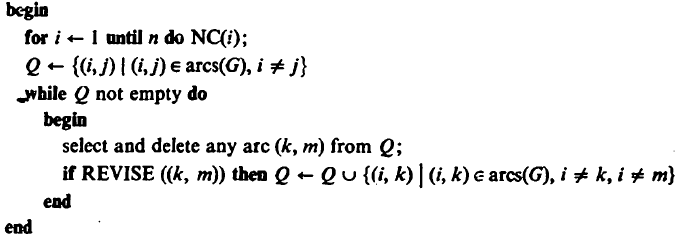
\includegraphics{AC3-AlanMackworth}
    \caption{Pseudocode AC-3 Algorithmus}\label{AC3}
\end{figure}
\begin{figure}[!htb]
    \centering
    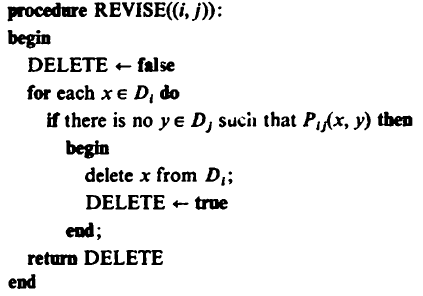
\includegraphics{Revise_AlanMackworth}
    \caption{Pseudocode Revise Algorithmus}\label{Revise}
\end{figure}

Der AC-3 Algorithmus beginnt mit Node Consistency ($NC(i)$). Diese ist bereits durch das Aufdecken gegeben und es können sich direkt mit den
binären Constraints beschäftigt werden. In meiner Implementierung beinhaltet die $Q$ die erzeugten binären Constraints. Für jede Kante wird
dann \textit{Revise} ausgeführt. Gibt es in \textit{Revise} eine Änderung, kann der übrig gebliebene Wert direkt gesetzt werden da der 
Wertebereich nur aus 0 und 1 besteht. Haben wir hier eine Mine gefunden, kann diese auch für das Spiel direkt markiert (mit einer Flagge)
werden. Alle Nachbarn von $k$ werden dann in $Q$ hinzugefügt. Desweiteren findet hier eine Überprüfung statt, ob die Variable $(xk, yk)$ bereits
konsistent ist (Referenz Konsistenz). Ist dies der Fall, sind alle benachbarten Felder mit dem Wert 0 sicher und können aufgedeckt werden.
Ist $Q$ leer, wird erst geschaut, ob das Spiel vorbei ist, nämlich genau dann wenn eine Mine oder alle Felder, die keine Mine sind, aufgedeckt
wurden. In dem Fall sind wir bereits fertig und können beenden. Ansonsten wird geschaut, ob sichere Felder zum Aufdecken hinzugefügt wurden
und von vorne begonnen. Sind wir hier durch, aber nicht fertig geht es mit 3. weiter.

Der Revise-Algorithmus schaut sich die Kanten/ binären Constraints an und prüft auf mögliche Verletzung der Constraints. Es wird jeder Wert
von $i$ der Kante $(i,j)$ bzw. $((xi, yi), (xj, yj))$ probeweise gesetzt und geschaut, ob dies dazu führt, dass $j$ keinen Wert annehmen kann,
der diesen Constraint erfüllen könnte. In dem Fall wird der getestete Wert für $i$ gelöscht und $DELETE$ auf \textit{false} gesetzt. Der Test
auf Verletzung dieses Constraints wird wie folgt durchgeführt: Für jeden Wert im Wertebereich von $j$ wird geschaut, ob dies seinen Constraint
zu allen Nachbarn verletzt. Dies kann der Fall sein, wenn für einen Nachbarn zu viele oder zu wenig Minen existieren würden, also die Summe
der Werte aller Nachbarn größer der Konstante ist oder die Anzahl der unbestimmten Nachbarn nicht mehr die erforderliche Anzahl an Minen 
erreichen könnten. 
Für \textit{Revise} muss beachtet werden, dass wir die Konstante von $j$ bei $(i,j)$ wissen müssen, das Feld also aufgedeckt sein muss. Ist
das nicht der Fall, wird diese Kante einfach übersprungen.

Nach 2. und vor 3. kommt in meinem Algorithmus noch ein Zwischenschritt. Da immer wieder zu AC-3 zurückgekehrt wird, kann es sein, dass bereits
alle Minen gefunden wurden. Tritt der Fall ein, können die restlichen Felder einfach aufgedeckt und der \textit{Solver} vollständig
konsistent gemacht werden. Dann ist der Algorithmus ebenfalls abgeschlossen. Ansonsten geht es bei [Backtracking] weiter.

\subsubsection{Backtracking}

Ist keine Lösung durch AC-3 gefunden worden, kommt Backtracking zum Einsatz, wie er auch in Quelle[y] beschrieben wird. Hierbei geht es darum,
für alle nicht belegten Variablen alle möglichen Zuweisungen zu generieren, testen und gültige zu sammeln. Schon bei kleinen Wertebereichen
führt dies zu einer hohen Komplexität. Im unserem Fall mit einem Wertebereich der Größe 2, liegt die Komplexität bei $\mathcal{O}(2^n)$.
Bei einem Minesweeper-Spielfeld für die Schwierigkeit \textit{Beginner} (8x8 mit 10 Minen) nimmt die Komplexität häufig ungewollte Ausmaße an.
Um dem entgegenzuwirken, wurden folgende Maßnahmen getroffen:
\begin{enumerate}
    \item Um nicht alle Möglichkeiten zu generieren und dann zu testen, wird vorzeitig abgebrochen, falls eine Zuweisung nicht gültig sein
    kann. Dies tritt beispielsweise ein, wenn die Summe der Werte in der Zuweisung größer als die Anzahl der übrigen Minen ist. Umgesetzt wird
    dies rekursiv aus Effizienz- und Lesbarkeitsgründen.
    \item Da viele Berechnungen durchgeführt werden, bei Tests auf Gültigkeit, wird \textit{Memoization} eingesetzt, also eine Art Cache eingeführt,
    für bereits berechnete Lösungen. 
    \item Um die Komplexität weiter zu reduzieren, werden außerdem Heuristiken festgelegt und genutzt. Da es regelmäßig vorkommt, dass ein
    Großteil der unbelegten Variablen keine aufgedeckten Nachbarn haben und damit wenig über die Gültigkeit einer Zuweisung dieser Variablen
    gesagt werden kann, werden diese exkludiert. In die Menge der Variablen, die für Backtracking angeschaut werden, kommen also nur solche,
    welche mind. einen Nachbar besitzen, der aufgedeckt ist. Desweiteren werden davon nur maximal 10 Variablen genommen, um die Komplexität
    auf $\mathcal{O}(2^{10})$ zu begrenzen.
\end{enumerate}

Wie werden Zuweisungen nun auf Gültigkeit geprüft?\\
Zuerst werden nur die Zuweisungen genommen, wo die Summe der Werte zwischen 1 und Anzahl Minen liegt bzw. gleich Anz. Minen ist, wenn es
sich um die letzen Felder/ Variablen handelt. Diese Unterscheidung beschreibt, dass die übrigen Minen nicht alle auf oder neben den gerade
betrachteten Feldern liegen müssen, sondern noch weiter außerhalb sein können. Wenn es sich um die letzten Felder handelt, müssen sich die
Minen offensichtlich unter denen befinden. Beispielsweise für den Fall, dass in der oberen linken Ecke eine 1 aufgedeckt wurde und Lösungen
generiert werden sollen, 3 mögliche Zuweisungen enstehen, nämlich dass genau ein Nachbar die Mine haben könnte.
Alle damit gültigen Zuweisungen werden dann weiter überprüft, in dem alle Werte probeweise gesetzt werden und auf Verletzung ihrer Constraints
geprüft wird. Wird nur der Constraint einer Variablen verletzt, ist die gesamte Zuweisung ungültig und wird verworfen. Andernfalls ist sie
gültig und kann zu der Menge der gültigen Lösungen hinzugefügt werden. An dieser Stelle werden dann auch Berechnungen in den Cache getan, 
zu Beginn der Lösungsüberprüfung abgefragt und regelmäßig aktualisiert (da sich das Spielfeld und damit die Umstände dynamisch ändern).

Wie wird mit den gültigen Zuweisungen umgegangen?\\
Je nachdem, wie viele Lösungen generiert worden sind, wird unterschiedlich weiter verfahren.
\begin{enumerate}
    \item \textbf{Es wurde keine gültige Lösung gefunden.} Konnte keine gültige Lösung gefunden werden, können wir nur damit weitermachen,
    ein zufälliges Feld auszuwählen und aufzudecken und anschließend wieder zu AC-3 zu gehen.
    \item \textbf{Es wurde genau eine gültige Lösung gefunden.} Konnte nur eine Lösung gefunden werden, dann kann direkt jedem der zugehörigen
    Variablen sein Wert zugewiesen werden. Hier zugewiesene Minen können markiert und sichere Felder aufgedeckt werden. Danach wird wieder
    [AC-3] ausgeführt. 
    \item \textbf{Es wurden mehrere gültige Lösungen gefunden.} Konnten mehrere Lösungen gefunden werden, werden diese zuerst gemeinsam betrachtet.
    Sollte es sichere Felder in jeder Lösung geben, also solche, für welche die Variable immer 0 ist, können diese aufgedeckt und zu AC-3
    zurückgekehrt werden. Gibt es jedoch kein sicheres Feld, wird die erste Lösung ausgewählt und alle dort als sicher markierten Felder
    aufgedeckt und auch zu AC-3 zurückgekehrt
\end{enumerate}

\subsection{Determinierung}

Der Algorithmus kann auf mehrere Arten determinieren. Folgend die Möglichkeiten:
\begin{enumerate}
    \item Der Algorithmus determiniert, weil das Spiel nach Minesweeper Regeln beendet ist. Dies ist entweder der Fall, wenn alle Felder aufgedeckt
    wurden, die keine Minen sind (es müssen nicht zwingend alle Minen markiert werden, dies ist im Grunde nur für die Orientierung eines menschlichen
    Spielers) oder eine Mine aufgedeckt wurde. Der Solver könnte eine Mine aufdecken, wenn bei der Lösungsfindung in Backtracking keine Lösung
    gefunden und folgend ein zufälliges Feld aufgedeckt wurde.
    \item Der Algorithmus determiniert, weil der Solver konsistent ist. In dem Fall müssen vorher nicht alle Felder aufgedeckt sein, werden
    es aber der Vollständigkeits halber vor Abschluss gemacht. Der Solver ist konsistent genau dann, wenn alle Variablen konsistent sind, 
    jede Variable einen Wert hat bzw. Wertebereich der Größe 1 und wenn die Summe der Variablen mit dem Wert 1 gleich der Anzahl der Minen ist.
    Variablen sind an sich konsistent, wenn sie als Mine markiert ist oder wenn die Summe der Werte der Variablen der Nachbarn gleich der
    Konstante $k$ dieser Variablen sind.
    \item Das Spiel ist nicht vorbei und der Solver ist nicht konsistent, aber alle Minen sind markiert und es existieren noch verdeckte Felder.
    Dann werden diese einfach aufgedeckt, bekommen ihre Werte zugewiesen und der Solver ist anschließend konsistent. Dies spart eine womöglich
    aufwändige Lösungsgenerierung durch Backtracking, weil es ein trivialer Fall ist.
\end{enumerate}

% !TEX root = ../termpaper.tex
% @author Kjell May
%
\graphicspath{{chapters/images/}}
\section{Experimente und Ergebnisse}


% !TEX root = ../termpaper.tex
% @author Kjell May
%
\graphicspath{{chapters/images/}}
\section{Fazit und Aussicht}

In dieser Hausarbeit wurde ein Algorithmus entwickelt und vorgestellt, der versucht Minesweeper als Constraint Satisfaction Problem lösen
zu können. Es hat sich gezeigt, dass diese Version schnell an Grenzen stößt und nur sehr einfache Konfigurationen lösen kann. Der Solver
ließe sich an einigen Stellen sicherlich noch erweitern und verbessern. Man könnte beispielsweise bei Auswahl des nächsten Feldes als 
Heuristik Wahrscheinlichkeiten, dass ein Feld eine Mine ist, nehmen, um möglicherweise mehr Fortschritt erlangen und ein vorzeitiges
Ende verzögern zu können. Ein paar Beispiel für andere Ansätze und Untersuchungen:\\
David Becerra hat in seiner Bachelorthesis \cite{AlgoApproaches} intensiver verschiedene Ansätze ausprobiert und
ist zu deutlich besseren Ergebnissen gekommen. Der Benutzer \textit{DavidNHill} hat einen Solver geschrieben (siehe \cite{statistics}), der
bei jedem Klick die Wahrscheinlichkeit für ein sicheres Feld berechnet. Robert Massaioli hat einen Algorithmus geschrieben, der Minesweeper
mit einem Matrizen-Ansatz löst (siehe \cite{matrix}). Aus einer Kombination der verschiedenen Ansätze könnte ein womöglich
effizienterer Algorithmus entwickelt werden.
Wie jedoch in \cite{MS-NP} und \cite{MS-Conf} von Richard Kaye gezeigt wurde, ist Minesweeper NP-complete und damit
ein effizienter Algorithmus zum Lösen dieses Spiel zu finden, sehr herausfordernd.


%\bibliographystyle{plain}
%\bibliographystyle{dinat}
\bibliographystyle{unsrtnat}
\clearpage
\bibliography{literature}

\Istatement

\end{document}
